\section{Abstract Interpretation}

For the following section we're following Mine's notes on abstract
interpretation \cite{mine:course}.

\begin{definition}[Galois connection]
  \label{def:galoisconn}
  A \emph{Galois connection} is a tuple \((\alpha, C, A, \gamma)\)
  where
  \begin{enumerate}
  \item \(A,C\) are complete lattices
  \item \(\alpha : C \to A\), \(\gamma : A \to C\) are a monotone
    \emph{abstraction} and \emph{concretization} maps.
  \item \(\forall a \in A, c\in C\) we have that \(c \sqsubseteq_C
    \gamma(a) \iff a \sqsubseteq_A \alpha(c)\)
  \end{enumerate}
\end{definition}

We're biulding a mapping between an \emph{abstract domain} \(A\) and a
\emph{concrete domain} \(C\), where the concretization and abstraction
maps \(\alpha, \gamma\) are sound, a visual rapresentation is in
figure \ref{fig:abstract}.

\begin{figure}
  \centering
  \usetikzlibrary {arrows.meta}
  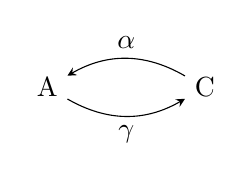
\begin{tikzpicture}[->, >=stealth]
    % Nodes
    \node (A) at (0,0) {A};
    \node (C) at (2,0) {C};
    
    % Arrows
    \path
    (C) edge[bend right=30] node[above]{$\alpha$} (A)
    (A) edge[bend right=30] node[below]{$\gamma$} (C);
  \end{tikzpicture}
  \caption{Galois connection between an abstract domain \(A\) and a
    concrete domain \(C\)}\label{fig:abstract}
\end{figure}

\begin{definition}[Galois Insertion]
  A Galois connection \((\alpha, C, A, \gamma)\) is a \emph{Galois
  Insertion} if one of the (equivalent) following conditions hold:
  \begin{enumerate}
  \item \(\alpha\) is surjective;
  \item \(\gamma\) is injective;
  \item \(\forall a \in A \quad \alpha(\gamma(a)) = a\)
  \end{enumerate}
\end{definition}

The intuition is that \(\alpha\) is a bijection, whose inverse
function is \(\gamma\), this way the abstract and the concrete domain
have the same cardinality, and therefore there are no ``useless''
abstract values.

\begin{definition}[Abstract domain]
  An \emph{abstract domain} is a tuple \((D^\sharp ,
  \sqsubseteq^\sharp, \gamma)\):
  \begin{itemize}
  \item a denumerable set \(D^\sharp\) of abstract values;
  \item a partial order \(\sqsubseteq^\sharp\) on \(D^\sharp\);
  \item a monotone concretization map \(\gamma : D^\sharp \to D\).
  \end{itemize}
  We denote with \(\bot^\sharp \in D^\sharp\) the smallest element of
  the abstract domain. Similarly, with \(\top^\sharp \in D^\sharp\) we
  rapresent the biggest element of the abstract domain. The
  concretization function sould express the map \(\gamma(\bot^\sharp)
  = \emptyset\) and \(\gamma(\top^\sharp) = \env\).
\end{definition}
